\documentclass[12pt]{article}

\usepackage[margin=1in]{geometry}
\usepackage{fancyhdr}
\pagestyle{fancy}
\usepackage{amsmath}
\usepackage{amssymb}
\usepackage{color}
\usepackage{enumerate}

\definecolor{mygreen}{rgb}{0,0.6,0}
\definecolor{mygray}{rgb}{0.5,0.5,0.5}
\definecolor{mymauve}{rgb}{0.58,0,0.82}
\definecolor{mylilas}{RGB}{170,55,241}
\usepackage{graphicx}
\usepackage{listings}
\lstset{language=Matlab,%
    %basicstyle=\color{red},
    frame=single, 
    breaklines=true,%
    morekeywords={matlab2tikz},
    keywordstyle=\color{blue},%
    morekeywords=[2]{1}, keywordstyle=[2]{\color{black}},
    identifierstyle=\color{black},%
    stringstyle=\color{mylilas},
    commentstyle=\color{mygreen},%
    showstringspaces=false,%without this there will be a symbol in the places where there is a space
    numbers=left,%
    flexiblecolumns=true,
    numbersep=9pt, % this defines how far the numbers are from the text
    emph=[1]{for,end,break},emphstyle=[1]\color{red}, %some words to emphasise
    %emph=[2]{word1,word2}, emphstyle=[2]{style}, 
    stepnumber=1  
}
\allowdisplaybreaks

\lhead{\Large 5168 Final Project}
\chead{\Large Melvyn Ian Drag}
\rhead{\Large\today}
\setlength{\parskip}{0pt} 
\setlength{\parindent}{0pt}
\newcommand{\tab}[1]{\hspace*{4ex}\rlap{#1}}
\newcommand{\tbf}[1]{\textbf{#1}}
\newcommand{\ptl}[2]{\frac{\partial^2 #1}{\partial #2 ^2}}
\newcommand{\der}[2]{\frac{d #1}{d #2}}
\newcommand{\iab}[2]{\int_{ #1 }^{ #2 }}
\newcommand{\rint}[1]{\int_1^{10} #1 dr}

\begin{document}
% Problem 1.1 -------------------------------------------------------
\section*{Problem One Point One}
\begin{center}
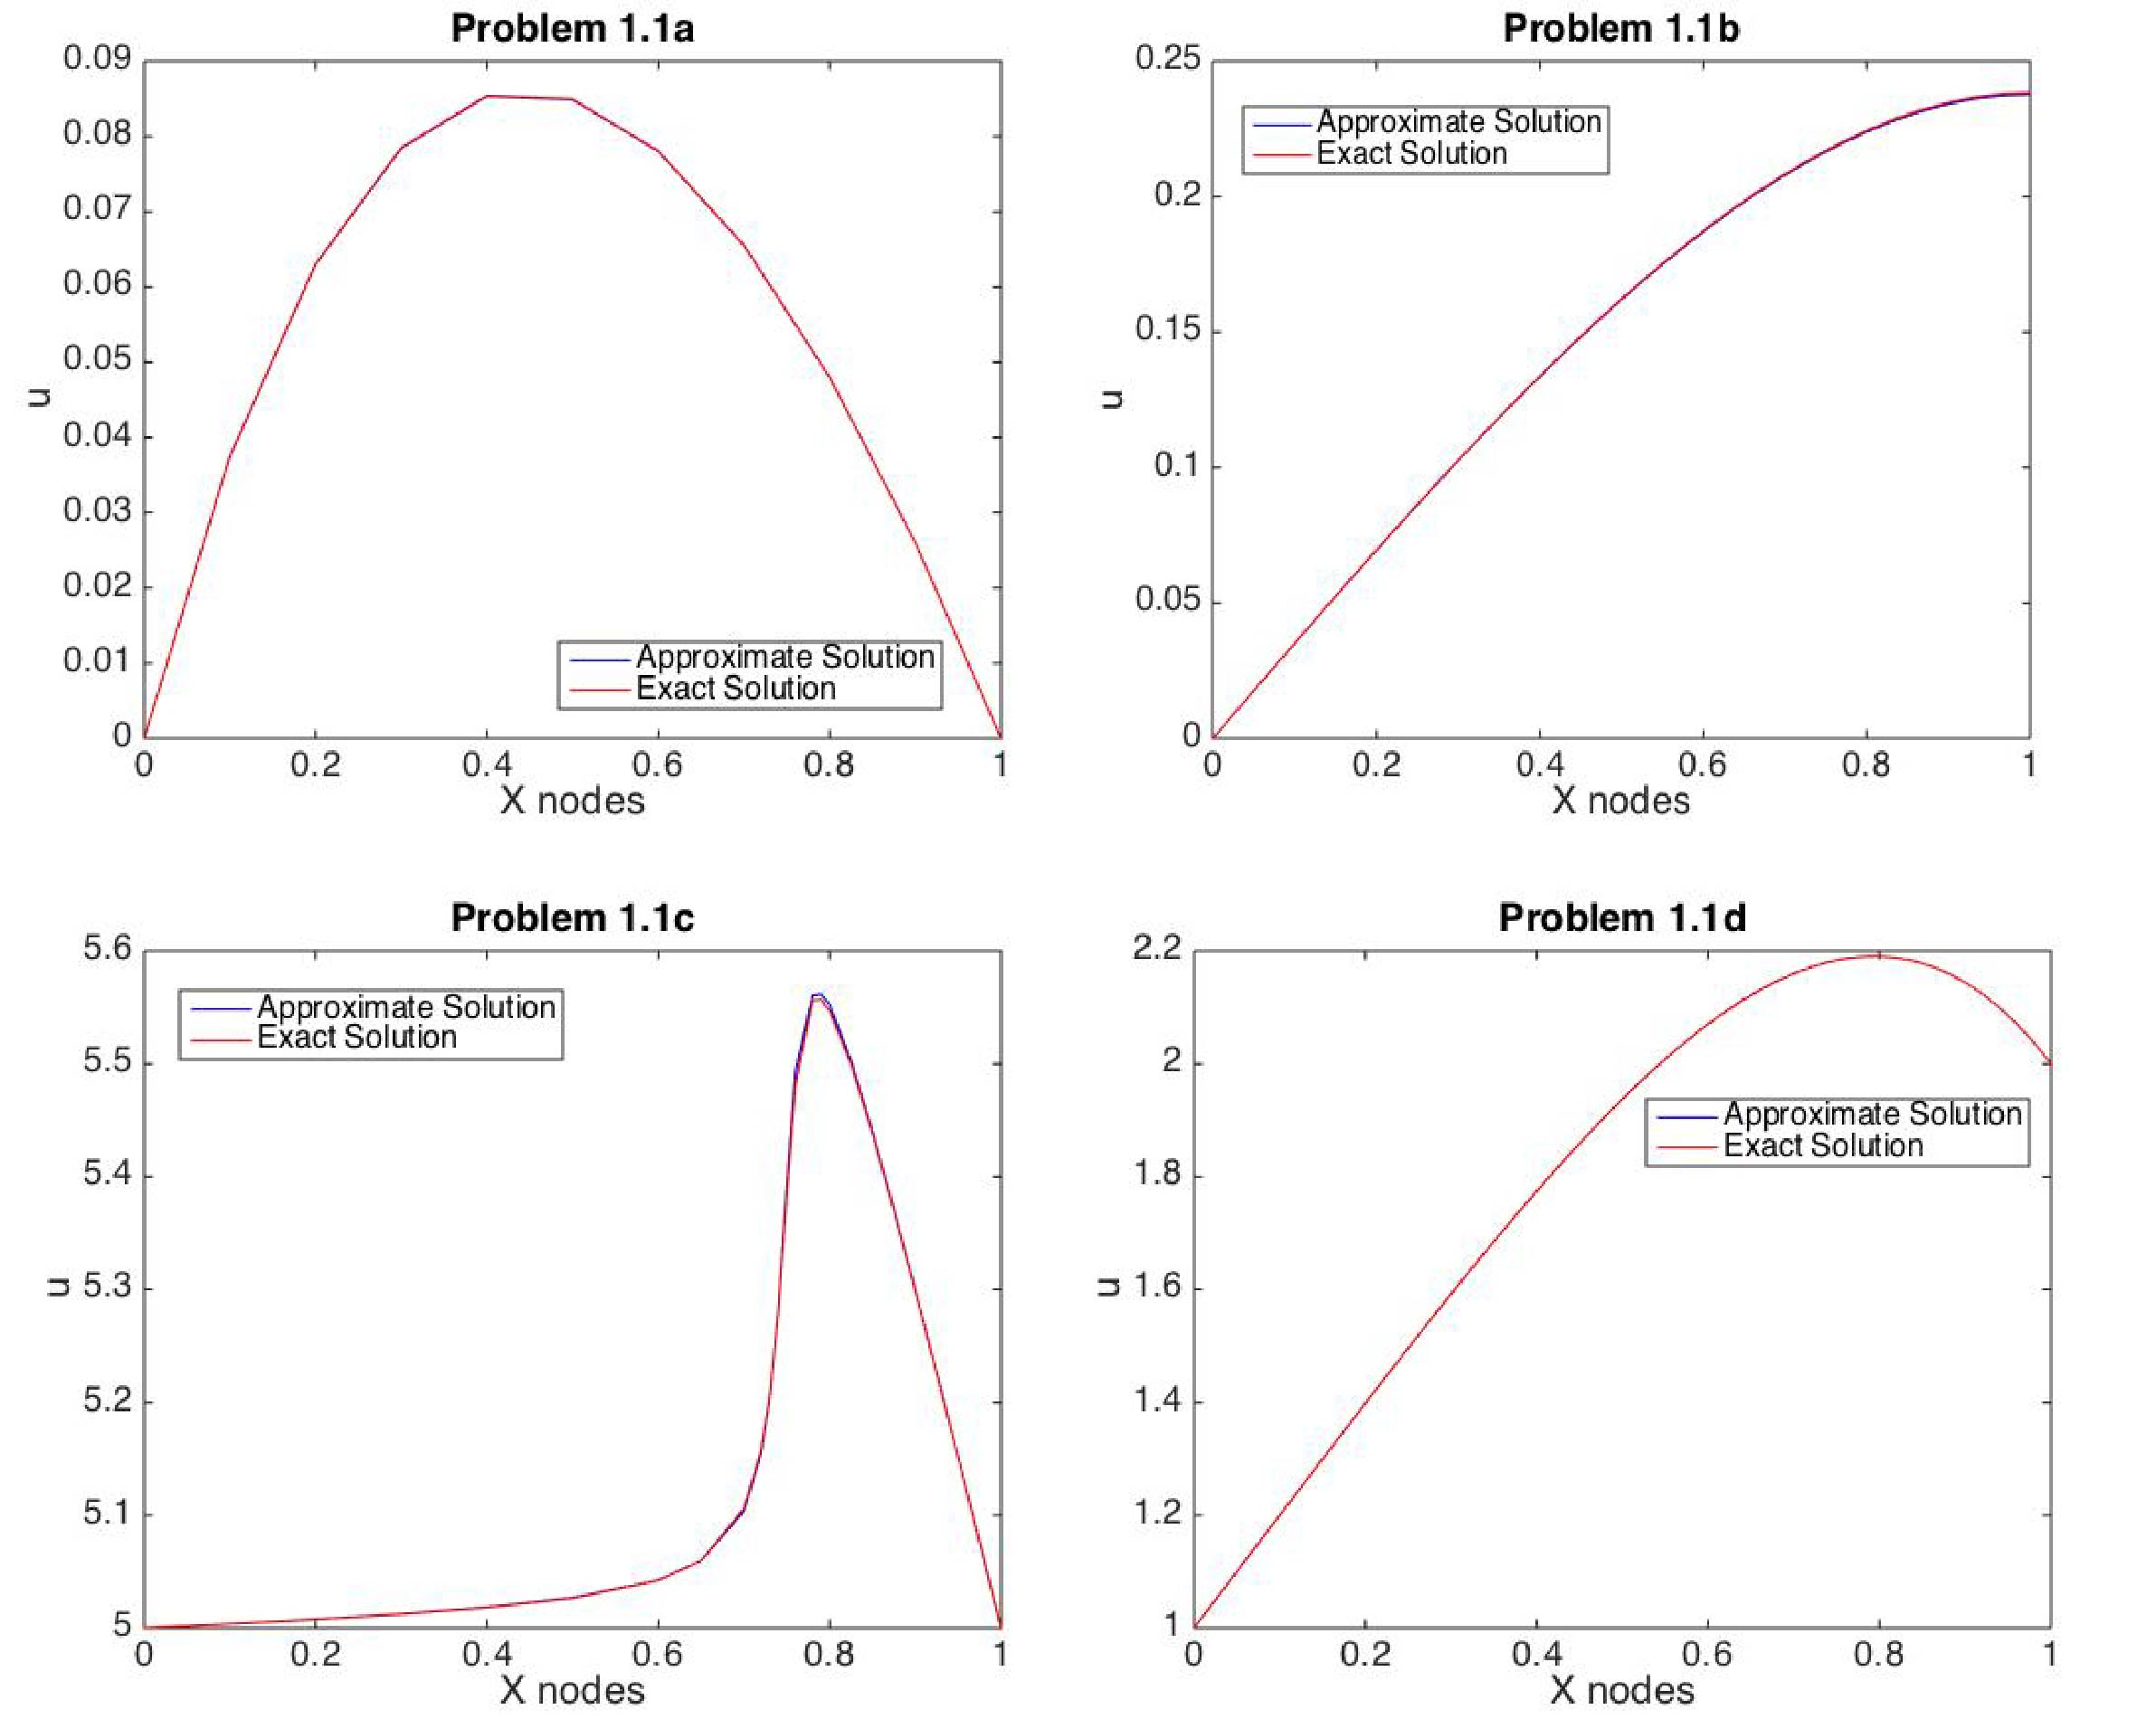
\includegraphics[width=\textwidth, keepaspectratio]{prob1.jpg}
\end{center}
% Problem 1.2 -------------------------------------------------------
\section*{Problem One Point Two}
\begin{enumerate}[(a)]
% 1.2a -------------------------------------------------------------
\item 
The strong form is given by:
\emph{Find $u\in C^2$ where}
\begin{gather*}
-\frac{d}{dr}(\kappa r\frac{du}{dr}) = rf\\
u(1) = 100,\;\;\; u(10) = 0
\end{gather*}

The weak form is derived at the end of the following steps:
\begin{gather*}
-\frac{d}{dr}(\kappa r\frac{du}{dr}) = rf\\
-\frac{d}{dr}(\kappa r\frac{du}{dr})\phi = rf\phi\\
-\rint{\frac{d}{dr}(\kappa r\frac{du}{dr})\phi} = \rint{rf\phi}\\
-\kappa\left(\phi r u_r\Big|_1^{10} - \rint{ru_r\phi_r}\right) = f\rint{r\phi}\\
\kappa\rint{ru_r\phi_r} = f\rint{r\phi}
\end{gather*}

% 1.2b --------------------------------------------------------------
\item If we are referring to \emph{relative error}, we get the desired accuracy with \texttt{Mesh 1}. The relative error at the indicated point is given by 
\begin{equation*}
\frac{|51.1219 - 48.8117|}{|51.1219|} = 0.0473 < \frac1{10}
\end{equation*}
There are 4 elements in this mesh. I'm quite sure that we are after the absolute error, however. we get the desired accuracy for \texttt{Mesh 4}.
\begin{equation*}
|(u - u_h)(3.25)| = |48.8679 - 48.8117| = 0.0562 < \frac1{10}
\end{equation*}
There are 32 elements in this mesh.
% 1.2c --------------------------------------------------------------
\item Here is the plot:

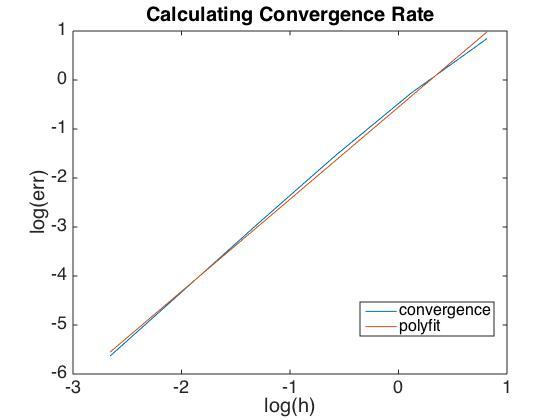
\includegraphics[width=0.5\textwidth]{prob12b.jpg}

Here is the code for plotting:
\begin{lstlisting}
err = fliplr(log([2.3102 0.7667 0.2162 0.0562 0.0142 0.0036]));
h = fliplr(log([2.25 1.125 0.5625 0.281250 0.140625 0.070312]));
p = polyfit(h, err, 1); % Fit to a line
disp(p(1));
P = polyval(p, h);
set(gcf, 'color', 'w')
plot(h, err, h, P)
title('Calculating Convergence Rate')
xlabel('log(h)')
ylabel('log(err)')
legend('convergence', 'polyfit')
\end{lstlisting}

The slope of the line given by \texttt{polyfit()} is $1.8811 \approx 2$.	

% 1.2d --------------------------------------------------------------
\item The absolute error in this example is $0.0459 < \frac1{10}$ at the indicated point. There are, however, only 10 elements, which is fewer than the 32 used in the structured mesh in part (b). The nodes are spaced more closely around $r = 3.25$ in the unstructured mesh than in some of the structured meshes with more elements, and therefore gives a better approximation in this neighborhood. 

Also, the solution is nearly linear in the right half of the domain, and so the solutions rapidly converge  point-wise for all meshes in this subdomain.  The unstructured mesh has nodes at only $x = 5.5$ and $x = 7.375$ and one of the structured meshes has nodes at $x = 6.625$, $x = 7.1875$, $x =7.75$, and $x =8.31$, yet both have similar accuracies in this neighborhood.
% 1.2e --------------------------------------------------------------
\item For this problem, I will use a finite difference to approximate $u_h'$ at the end points. That is, the derivative is approximated as
\begin{equation*}
u_h' = \frac{u^{(e)}_l- u^{(e)}_r}{h^{(e)}}
\end{equation*}
where $e$ denotes `element', $l$ denotes `left' and $r$ denotes `right' for the left and right endpoints of the element. Since we are looking for $10\%$ error, I assume that in this case we are referring to relative error and not absolute error. At the left endpoint I get the desired accuracy with \texttt{Mesh 5}. At the right endpoint I get the desired accuracy with \texttt{Mesh 2}.
% 1.2f --------------------------------------------------------------
\item The convergence of the flux is slower than the convergence for the solution. The rates of convergence are about $0.7847$ and $1.1516$ at the left and right endpoints, respectively. 

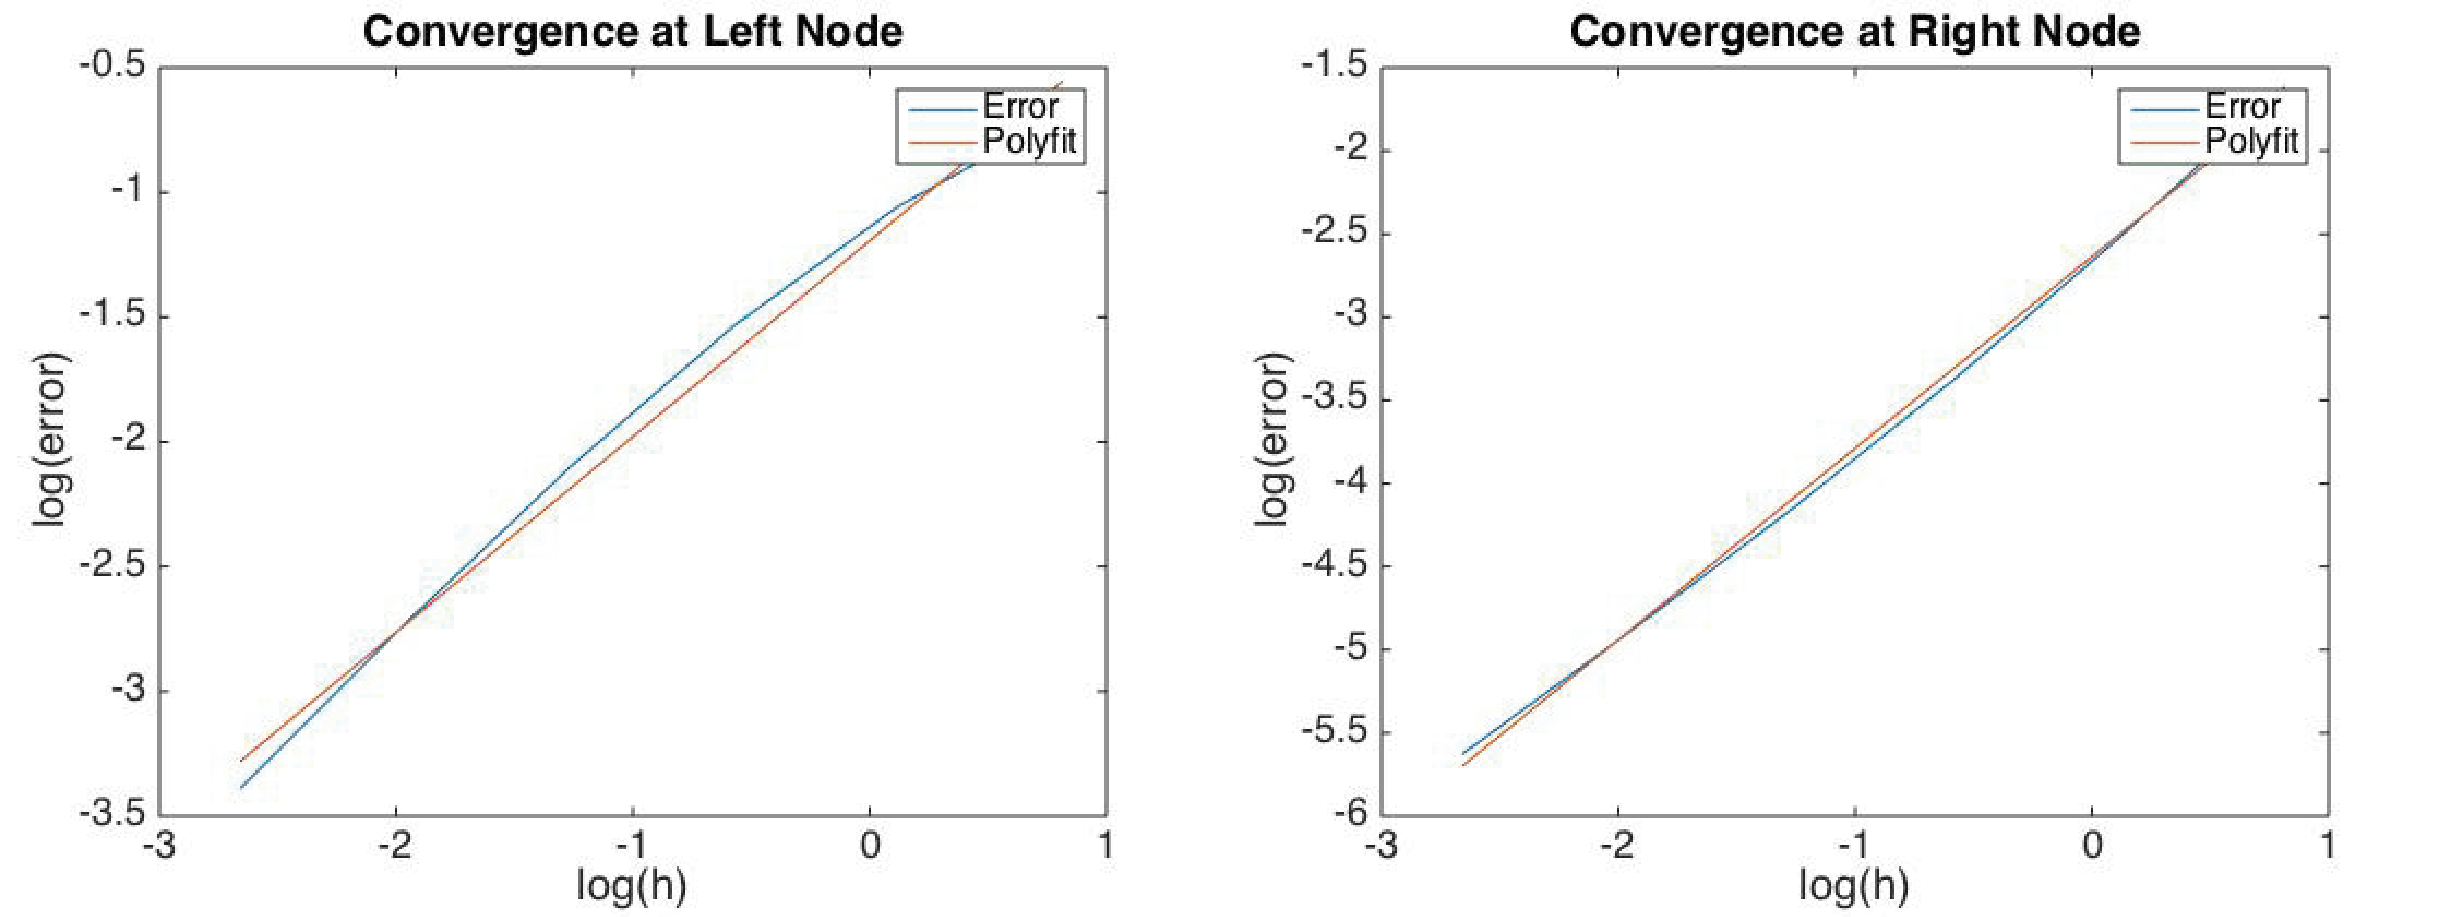
\includegraphics[width=\textwidth]{convergence.png}
\end{enumerate}
% Problem 2.1 -------------------------------------------------------
\section*{Problem Two Point One}
% Problem 2.2 -------------------------------------------------------
\section*{Problem Two Point Two}


\end{document}
